\documentclass[a4paper]{article}
\usepackage[a4paper,top=2cm,bottom=2cm,left=2cm,right=2cm,marginparwidth=2cm]{geometry}
\usepackage{lmodern}
\usepackage{listings}
\usepackage{amsmath}
\usepackage{amssymb}
\usepackage{bm}
\usepackage{graphicx}
\usepackage{textpos}
\usepackage{tcolorbox}
\usepackage{pgf,tikz}
\usetikzlibrary{arrows,automata}

\setlength{\parindent}{0em}
\setlength{\parskip}{0.3em}
\lstset{language=Python,upquote=true,basicstyle=\ttfamily\small,breaklines=true}

\begin{document}
\title{AICE3002/AICE6001 Laboratory Portfolio\\Investigation 2 -- Optimisation and Wide Networks}
\author{Jonathon Hare \& Antonia Marcu\\\{j.s.hare, a.marcu\}@soton.ac.uk}
\date{2026--27}
\maketitle

This is the second of four individual investigations that make up the laboratory portfolio. It should be completed after the optimisation, linear-model, and MLP practical work. You should write up your results, answers, and findings succinctly, and submit your executable notebook alongside the report.

You should use \emph{no more than two sides of A4} for this investigation. Code need not be reproduced in full: include only short snippets needed to explain your method. This investigation is worth 10 marks.

\section{Exploring optimisation of an analytic function}

The $d$-dimensional Rastrigin function is
\begin{equation}
f(\bm x)=Ad+\sum_{i=1}^{d}\left(x_i^2-A\cos(2\pi x_i)\right).
\end{equation}
It has a global minimum at the origin but also contains many local minima. For this exercise use $d=2$ and $A=0.5$.

\begin{figure}[h!]
    \centering
    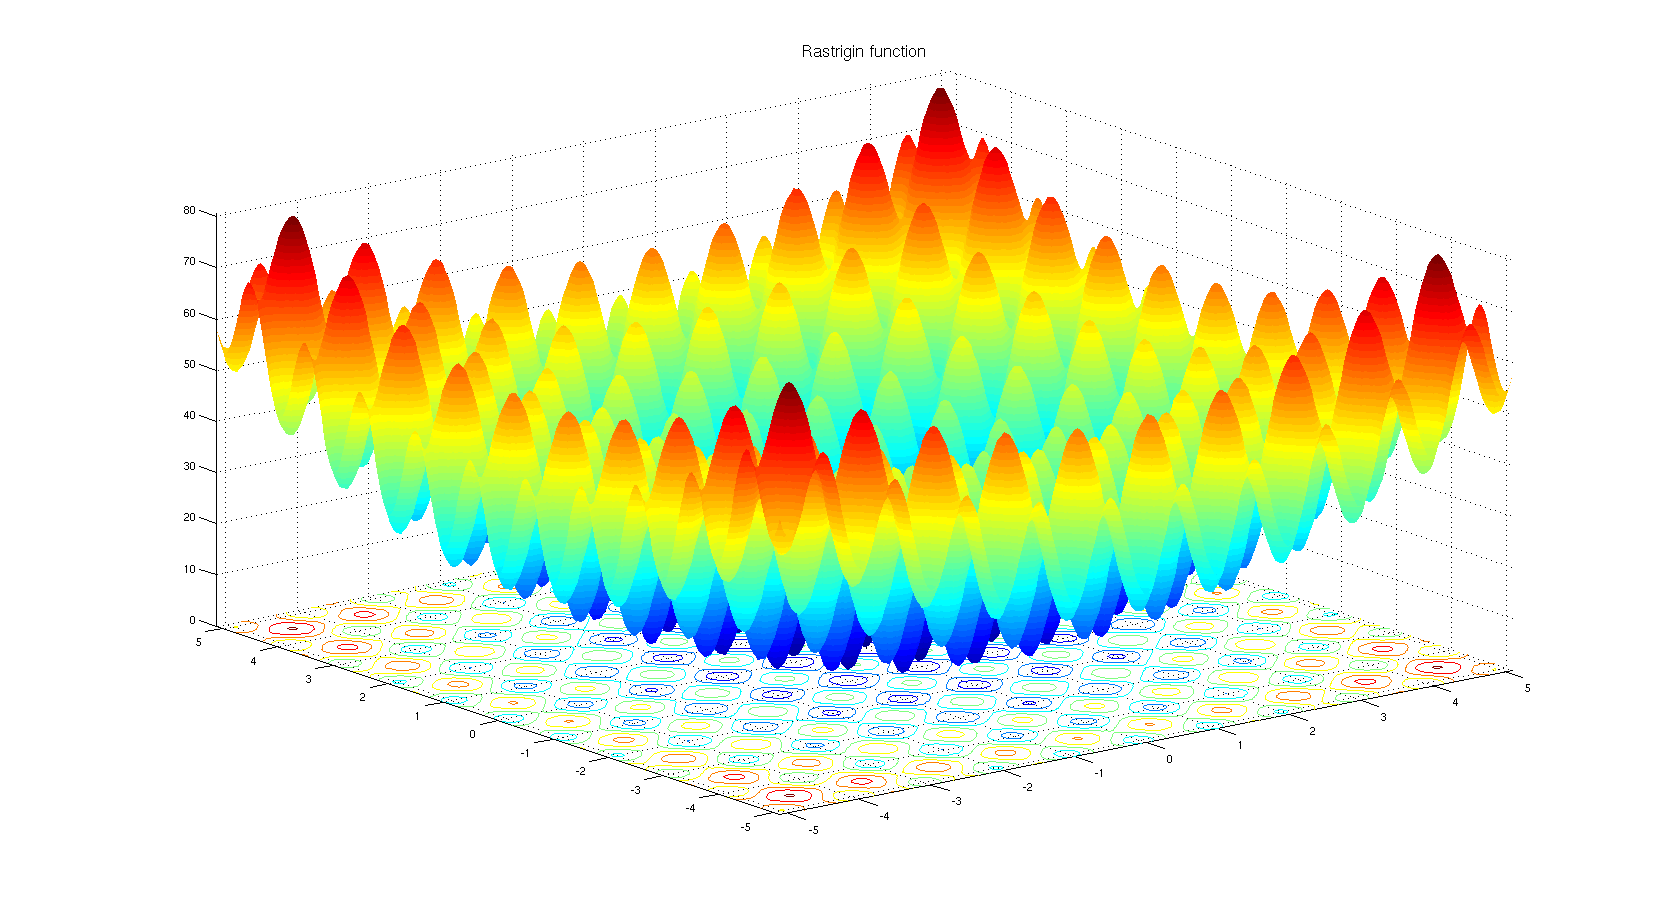
\includegraphics[width=0.72\textwidth]{Rastrigin_function.png}
    \caption{The Rastrigin function with the conventional $A=10$, illustrating its many local minima. The experiments below use the smoother $A=0.5$ surface.}
\end{figure}

\begin{tcolorbox}[title=1.1 Optimise the Rastrigin function (3 marks)]
Starting from $[5,4]^{\top}$, run each of the following PyTorch optimisers for 100 iterations:
\begin{itemize}
    \item SGD with learning rate 0.01;
    \item SGD with learning rate 0.01 and momentum 0.9;
    \item Adagrad with learning rate 0.01; and
    \item Adam with learning rate 0.01.
\end{itemize}
Use default values for unspecified parameters. Report the final point and function value for each optimiser, and plot loss against iteration on a common set of axes.
\end{tcolorbox}

\begin{tcolorbox}[title=1.2 Interpret the optimiser behaviour (2 marks)]
Which optimiser worked best in Task 1.1? Is that conclusion robust to a different starting point or a modest change in learning rate? Perform a small number of additional runs sufficient to support your answer, and explain the behaviour you observe in terms of the loss surface and update rules. Do not perform an exhaustive hyperparameter search.
\end{tcolorbox}

\section{Wide MLPs on MNIST}

In the lab exercise you built a \texttt{BaselineModel} which was a simple MLP with one hidden layer and trained it on MNIST. You're now going to explore this model further.

\begin{tcolorbox}[title=2.1 Wider MLPs (5 marks)]
Consider an MLP with a single hidden layer. How wide does the network need to be (how many hidden units) before it overfits\footnote{Fails to generalise \emph{reasonably} to the MNIST test set.} on the MNIST training dataset? Provide a rationale for your answer and experimental evidence for your findings, and suggest reasons why they might be so.

For practical purposes you are limited by available accelerator memory; do not try training networks with more than 500,000 hidden units, which have almost 400 million learnable parameters. For experimental evidence you should include training curves (plots of loss and accuracy against epochs) with both the training and test data for a range of differently sized models.
\end{tcolorbox}

\end{document}
